%%%%% Document Setup %%%%%%%%

\documentclass[10pt, twocolumn]{revtex4}    % Font size (10,11 or 12pt) and column number (one or two).

\usepackage{times}                          % Times New Roman font type

\usepackage[a4paper, left=1.85cm, right=1.85cm,
 top=1.85cm, bottom=1.85cm]{geometry}       % Defines paper size and margin length

\usepackage[font=small,
labelfont=bf]{caption}                      % Defines caption font size as 9pt and caption title bolded

\usepackage{mathtools,amssymb}
\usepackage{graphics,graphicx,epsfig,ulem}	% Makes sure all graphics works
\usepackage{amsmath} 						% Adds mathematical features for equations
%\usepackage{siunitx}
\usepackage{textcomp}
\usepackage{enumitem}
\usepackage{bm}
\usepackage{lipsum}
\usepackage[toc,page]{appendix}
\usepackage{booktabs}
\usepackage{rotating}
\usepackage{siunitx}
\usepackage{multirow}
\usepackage{ulem}
\usepackage{array}
\newcolumntype{L}[1]{>{\raggedright\arraybackslash}p{#1}}

\usepackage{etoolbox}                       % Customise date to preferred format
\makeatletter
\patchcmd{\frontmatter@RRAP@format}{(}{}{}{}
\patchcmd{\frontmatter@RRAP@format}{)}{}{}{}
\renewcommand\Dated@name{}
\newcommand{\rom}[1]{\uppercase\expandafter{\romannumeral #1\relax}}
\makeatother

%\usepackage[flushleft]{threeparttable}

\usepackage{fancyhdr}

\pagestyle{fancy}                           % Insert header
\renewcommand{\headrulewidth}{0pt}
\lhead{P. Einarsson Nielsen}                          % Your name
\rhead{TITLE}           % Your report title               

\def\bibsection{\section*{References}}        % Position refernce section correctly


\AtBeginDocument{
	\heavyrulewidth=.08em
	\lightrulewidth=.05em
	\cmidrulewidth=.03em
	\belowrulesep=.65ex
	\belowbottomsep=0pt
	\aboverulesep=.4ex
	\abovetopsep=0pt
	\cmidrulesep=\doublerulesep
	\cmidrulekern=.5em
	\defaultaddspace=.5em
}


%%%%% Document %%%%%
\begin{document}                     


\title{TITLE} 
\date{Submitted: \today{}}
\author{P. Einarsson Nielsen}
\affiliation{\normalfont Affiliation}

\begin{abstract}
	\lipsum[1]

\end{abstract}

\maketitle
\thispagestyle{plain} % produces page number for front page



\section{Introduction} \label{s:intro}

\begin{itemize}
	\item Detail balance
	\item Ergodic
	\item Stochastic
	\item Entropy driven phase transitions
	\item Equations of state
	
\end{itemize}

%\lipsum[1-8]

%\subsection{Subsection} \label{ss}
%\lipsum[1-3]


\section{Methodology} \label{s:methods}
%\lipsum[1-10]

\section{Model} \label{s:model}
Our simulated system consists of $N$ number of particles enclosed in a cubic container of volume $V$. The potential energy between any two particles in the system is given by the Lennard-Jones potential, expressed in the reduced unit scheme as
\begin{equation}
U_{LJ} = 4\left(\frac{1}{r^{12}}-\frac{1}{r^{6}}\right)
\end{equation}
where $r$ is the reduced distance between the particles.
The number of particles in the system was kept constant for every initial configuration and, as such, achieving a given reduced density required the container length to be varied. When applying perturbations to a particle in the system, the interaction potential was considered for every other particle in the system under periodic boundary conditions, or up to half the container length.

Virial equation and configuration energy per particle


The model and method were verified by direct comparison to Monte Carlo results at liquid and vapour-like densities along isotherms $T^{*}=0.85, 0.90$ published by United States' National Institute of Standard and Technology (NIST). NIST's results were for 500 particles whose Lennard-Jones interaction had been truncated to $3\sigma{}$ and standard long range corrections had been applied. Their systems were equilibrated for $5.0\text{e}7$ moves and quantities calculated over $2.5\text{e}8$ moves. Figure \ref{fig:NIST_comparison} shows the configuration energy per particle, $u^*$, and virial pressure, $p^{*} = P - \rho{}kT$ for both our system and NIST's. Our results were obtained as described in section \ref{s:methods}.

\begin{figure}
	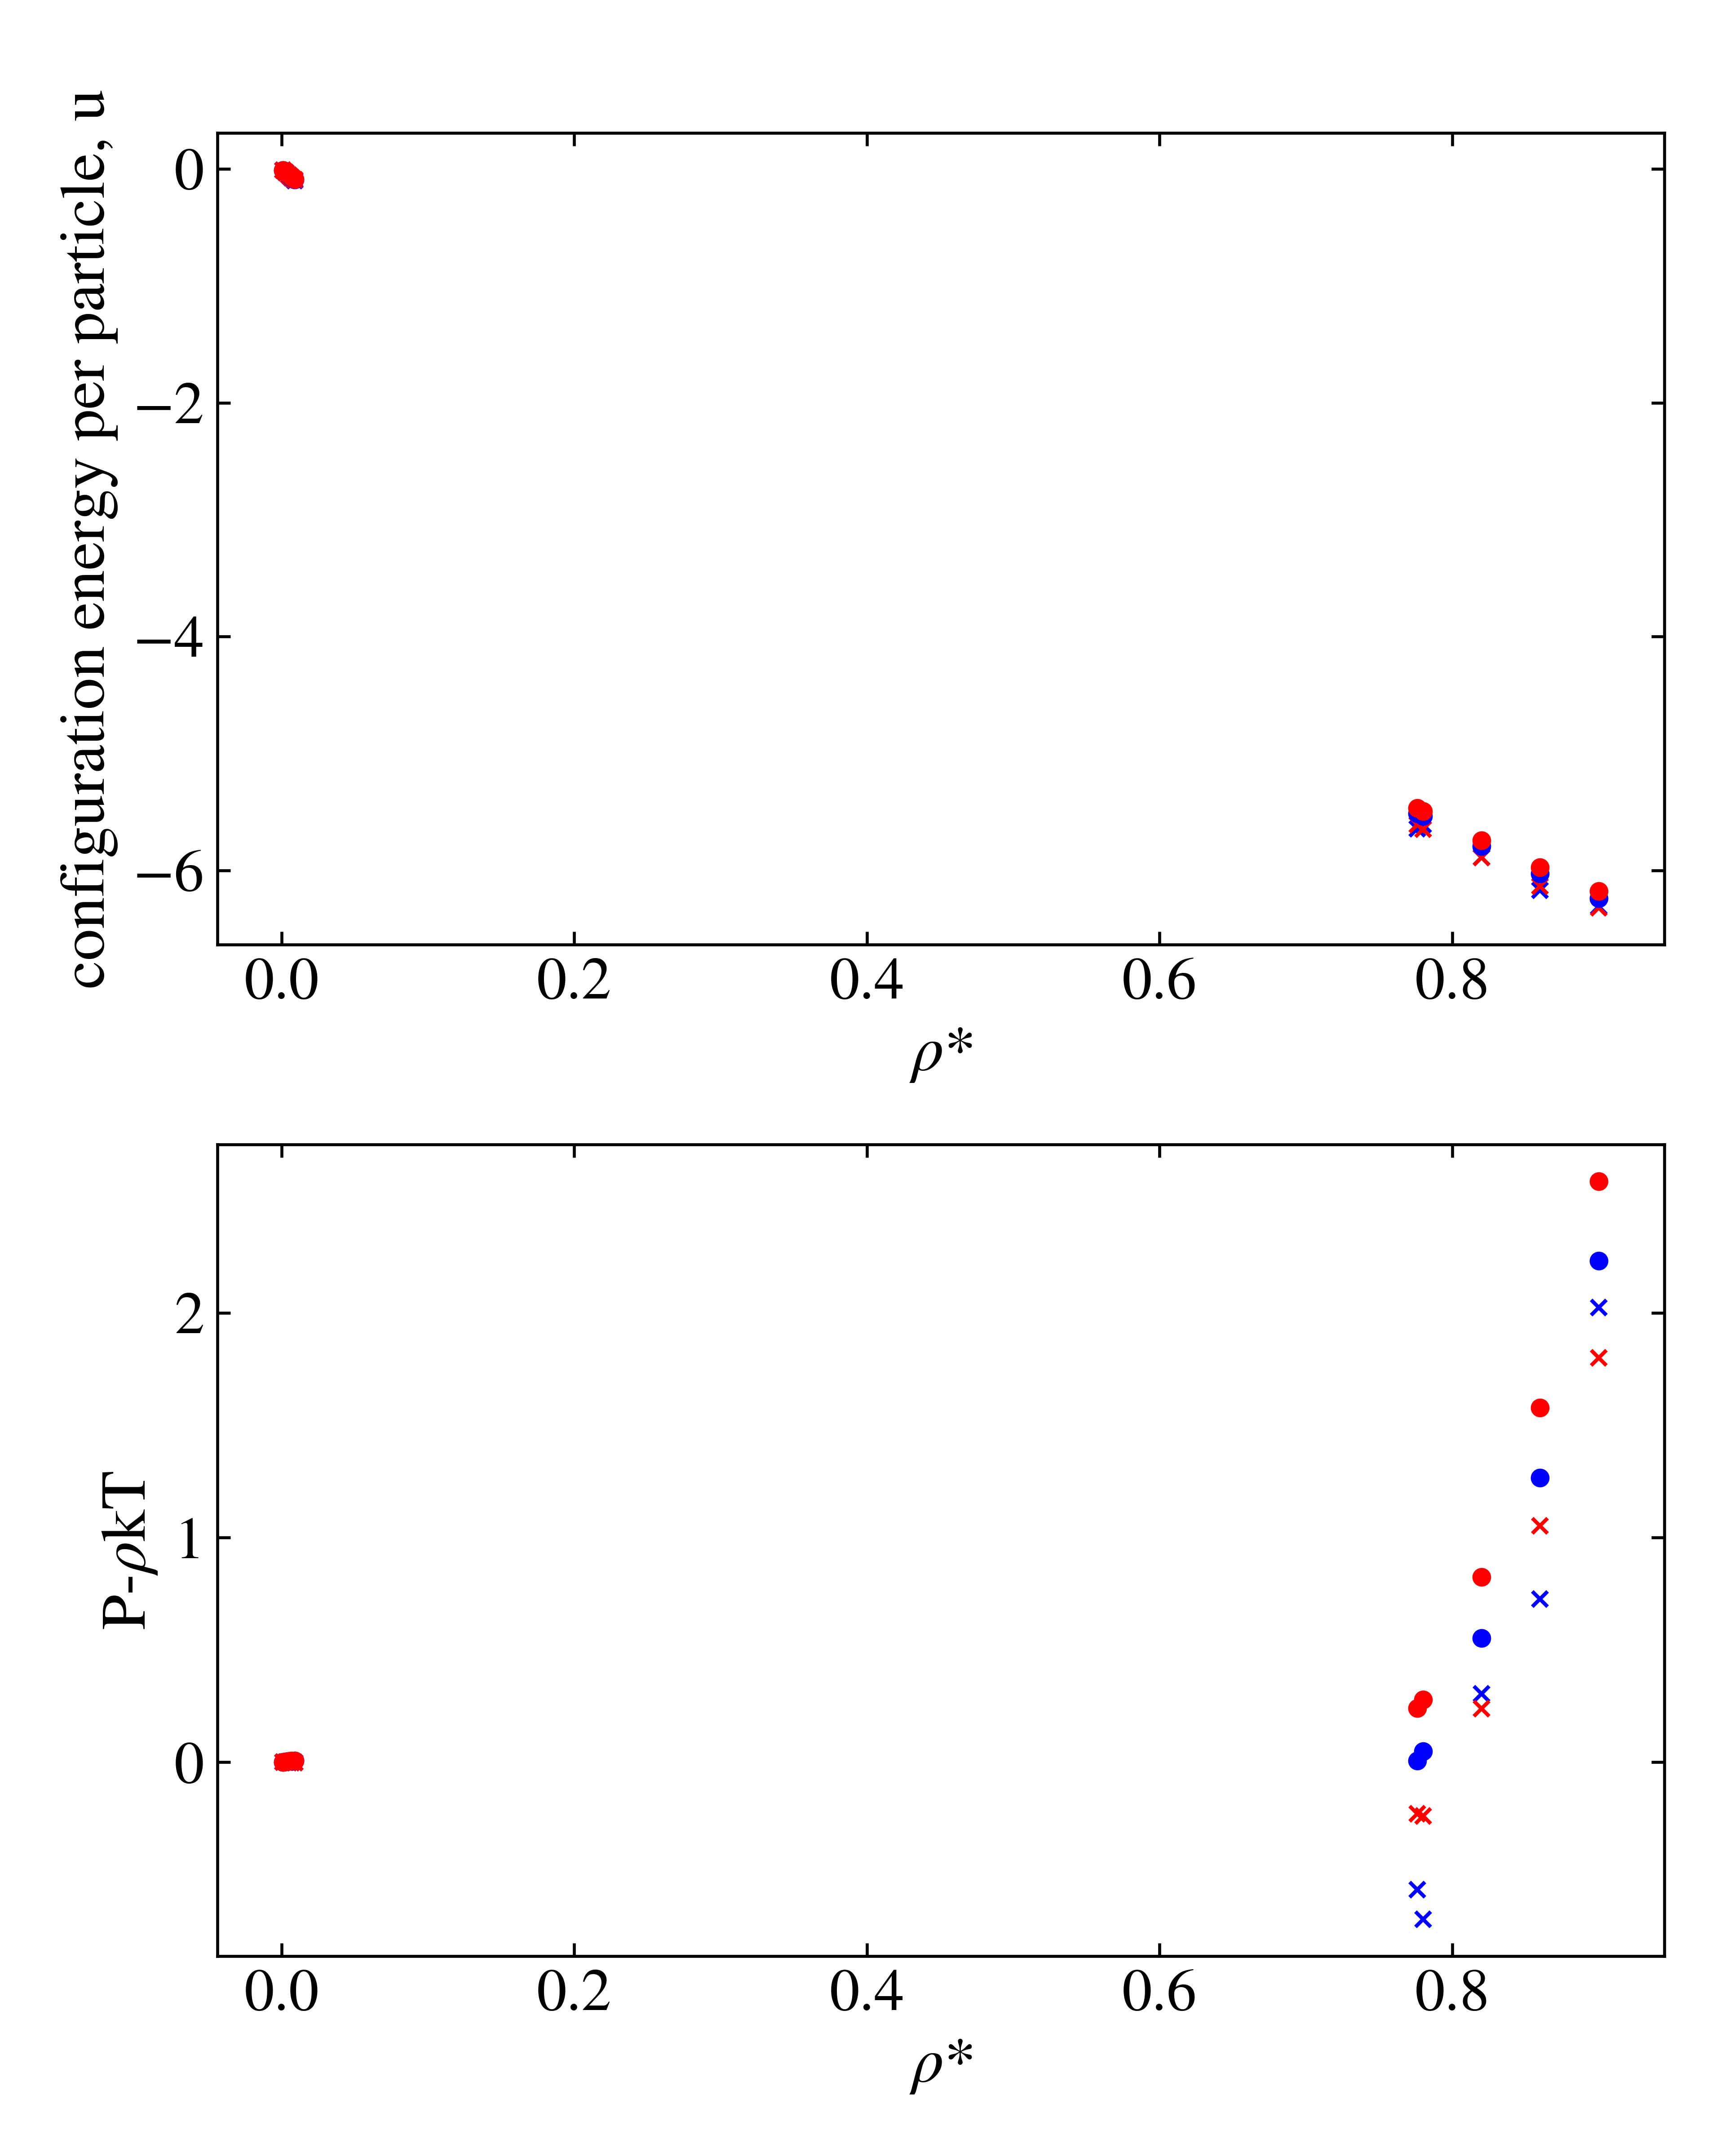
\includegraphics[width=\linewidth]{figures/NISTcomparison.png}
	\caption{Configuration energy per particle, $u^*$, and virial pressure, $p^{*} = P - \rho{}kT$ for NIST data (dots) and our model (crosses). The blue and red data are along isotherms $T^{*} = 0.85, 0.90$ respectively.}
	\label{fig:NIST_comparison}
\end{figure}



\section{Results} \label{s:results}
%\lipsum[1-10]

\section{Discussion} \label{s:analysis}
%\lipsum[1-15]


\section{Conclusions} \label{s:conclusions}
%\lipsum[1-5]

\begin{thebibliography}{}

\bibitem{ref01} A. N. Other, Title of the Book, edition, publishers, place of publication (year of publication), p. 123.   % example reference

\bibitem{errors}I. G. Hughes, T. P. A Hase, Measurements and their Uncertainties A Practical Guide to Modern Error Analysis, 1st, Oxford University Press, Oxford (2010)

\end{thebibliography} 

\clearpage
\appendix
\section{Error Analysis} \label{a:errors}
All propagation of errors is performed as outlined in \cite{errors}.

\clearpage
\section{Comparison to NIST data} \label{a:NIST}


% Please add the following required packages to your document preamble:
% \usepackage{booktabs}
% \usepackage{graphicx}
\begin{table}[]
	\resizebox{\textwidth}{!}{%
		\begin{tabular}{@{}llllllllll@{}}
			\toprule
			$T^*$    & $\rho{}^*$ & $U_\text{NIST}^*$ & $\pm$    & $U*$ & $\pm$ & $p_\text{NIST}^*$ & $\pm$    & $p^*$ & $\pm$ \\ \midrule
			8.50E-01 & 1.00E-03   & -1.0317E-02       & 2.34E-05 &      &       & 8.4402E-04        & 4.66E-08 &       &       \\
			8.50E-01 & 3.00E-03   & -3.1019E-02       & 5.91E-05 &      &       & 2.4965E-03        & 4.99E-07 &       &       \\
			8.50E-01 & 5.00E-03   & -5.1901E-02       & 7.53E-05 &      &       & 4.1003E-03        & 5.05E-07 &       &       \\ 
			8.50E-01 & 7.00E-03   & -7.2834E-02       & 1.34E-04 &      &       & 5.6565E-03        & 7.96E-07 &       &       \\
			8.50E-01 & 9.00E-03   & -9.3973E-02       & 1.29E-04 &      &       & 7.1641E-03        & 2.24E-06 &       &       \\
			8.50E-01 & 7.76E-01   & -5.5121E+00       & 4.55E-04 &      &       & 6.7714E-03        & 1.77E-03 &       &       \\
			8.50E-01 & 7.80E-01   & -5.5386E+00       & 7.26E-04 &      &       & 4.7924E-02        & 3.18E-03 &       &       \\
			8.50E-01 & 8.20E-01   & -5.7947E+00       & 6.03E-04 &      &       & 5.5355E-01        & 4.13E-03 &       &       \\
			8.50E-01 & 8.60E-01   & -6.0305E+00       & 2.38E-03 &      &       & 1.2660E+00        & 1.36E-02 &       &       \\
			8.50E-01 & 9.00E-01   & -6.2391E+00       & 5.27E-03 &      &       & 2.2314E+00        & 2.72E-02 &       &       \\ \midrule
			9.00E-01 & 1.00E-03   & -9.9165E-03       & 1.89E-05 &      &       & 8.9429E-04        & 2.48E-08 &       &       \\
			9.00E-01 & 3.00E-03   & -2.9787E-02       & 3.21E-05 &      &       & 2.6485E-03        & 2.54E-07 &       &       \\
			9.00E-01 & 5.00E-03   & -4.9771E-02       & 3.80E-05 &      &       & 4.3569E-03        & 2.19E-07 &       &       \\
			9.00E-01 & 7.00E-03   & -6.9805E-02       & 7.66E-05 &      &       & 6.0193E-03        & 1.02E-06 &       &       \\
			9.00E-01 & 9.00E-03   & -8.9936E-02       & 2.44E-05 &      &       & 7.6363E-03        & 1.44E-06 &       &       \\
			9.00E-01 & 7.76E-01   & -5.4689E+00       & 4.20E-04 &      &       & 2.4056E-01        & 2.74E-03 &       &       \\
			9.00E-01 & 7.80E-01   & -5.4956E+00       & 7.86E-04 &      &       & 2.7851E-01        & 2.97E-03 &       &       \\
			9.00E-01 & 8.20E-01   & -5.7456E+00       & 7.51E-04 &      &       & 8.2386E-01        & 2.85E-03 &       &       \\
			9.00E-01 & 8.60E-01   & -5.9753E+00       & 5.53E-04 &      &       & 1.5781E+00        & 3.29E-03 &       &       \\
			9.00E-01 & 9.00E-01   & -6.1773E+00       & 1.57E-03 &      &       & 2.5848E+00        & 9.54E-03 &       &       \\ \bottomrule
		\end{tabular}%
	}
\end{table}

\end{document}